\vspace{1cm}
\section{Strahlungsfelder und Antennen}
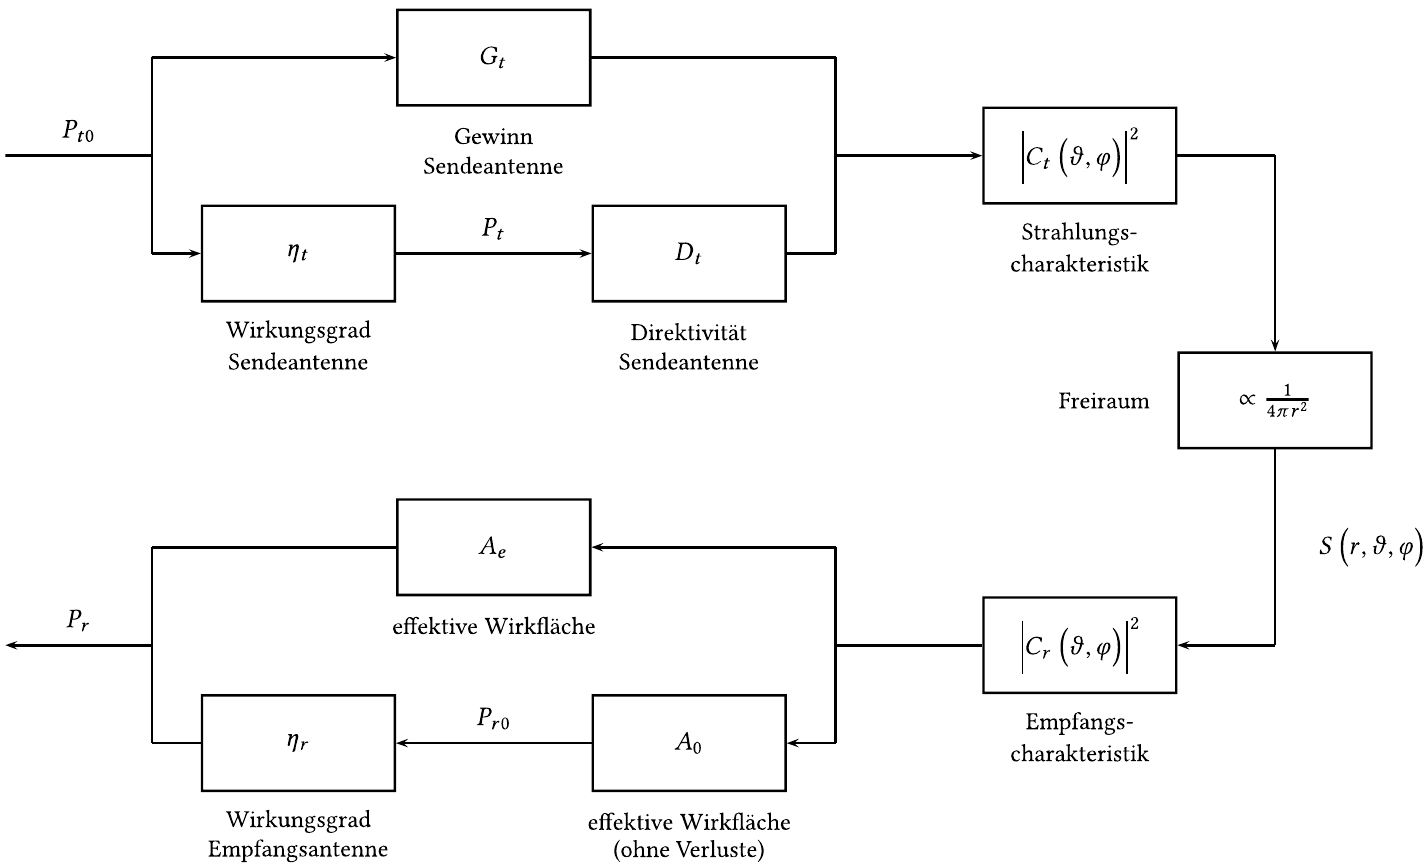
\includegraphics[width=.4\paperheight]{content/fuw/pictures/fuw_antenne.png}
\begin{itemize}
    \itemsep0pt
    \item Feldbereiche:
        \begin{itemize}
            \itemsep0pt
            \item \(r < \frac{\lambda}{2\pi}\): reaktives Nahfeld
            \item \(\frac{\lambda}{2\pi} < r < \frac{2D^2}{\lambda}\): strahlendes Nahfeld
            \item \(r > \frac{2D^2}{\lambda}\): Fernfeld
        \end{itemize}
    \item Effektive Wirkfläche \(A_e = \dfrac{\lambda^2}{\pi} G_r\)
    \item Sendeantenne optimal ausgerichtet:\\
        \(\left|C_r(\vartheta, \varphi)\right| = 1 \implies S(r,\vartheta,\varphi) = S_{\mathrm{max}}(r)\)
    \item Empfangsantenne optimal ausgerichtet:\\
        \(\left|C_r(\vartheta, \varphi)\right| = 1 \implies P_r = P_{r, \mathrm{max}}\)
    \item \textbf{Fernfeld:} \(r \gg \lambda \implies kr \gg 2\pi\)
    \item Senden:
        \begin{itemize}
            \itemsep0pt
            \item Gesendete Leistung (ohne Verluste) \(P_{t0}\)
            \item Gesendete Leistung \(P_t\)
            \item Leistungsflussdichte \(S(r, \vartheta, \varphi)\)
            \item Leistungsflussdichte (\textit{isotroper Kugelstrahler}) \(S_i(r) = \dfrac{P}{4\pi r^2}\)
            \item Strahlungscharakteristik \(C_t(\vartheta, \varphi) = \left.\dfrac{E(\vartheta, \varphi)}{E_{max}}\right|_{r = \mathrm{const}}\)
            \item Direktivität \(\left.D_t = \dfrac{S_{max}}{S_i}\right|_{P_t} = \dfrac{4\pi r^2 S_{max}}{P_{t}}\)
            \item Gewinn \(\left.G_t = \dfrac{S_{max}}{S_i}\right|_{P_{t0}} = \dfrac{4\pi r^2 S_{max}}{P_{t0}}\)
            \item Wirkungsgrad \(\eta_t = \dfrac{G_t}{D_t}\)
        \end{itemize}
    \item Empfangen:
        \begin{itemize}
            \itemsep0pt
            \item Empfangene Leistung (ohne Verluste) \(P_{r0}\)
            \item Empfangene Leistung \(P_r\)
            \item Empfangscharakteristik \(C_r(\vartheta, \varphi) = \left.\dfrac{U(\vartheta, \varphi)}{U_{max}}\right|_{S = \mathrm{const}}\)
            \item Effektive  Wirkfläche (ohne Verluste): \(A_0 = \dfrac{P_{r0,\mathrm{max}}}{S} = \dfrac{\lambda^2}{4\pi}D_r\)
            \item Effektive  Wirkfläche: \(A_e = \dfrac{P_{r,\mathrm{max}}}{S} = \dfrac{\lambda^2}{4\pi}G_r\)
            \item Wirkungsgrad \(\eta_r = \dfrac{A_e}{A_0}\)
        \end{itemize}

\end{itemize}
